\section{Trajectory Optimization}
\label{sec:trajectory_optimization}

A trajectory optimization is a set of mathematical techniques, which is used to find an ideal or the best behavior for a dynamic system, or also known as optimal trajectory. In order to describe mathematically what is understood as the "best" trajectory, an \emph{objective function} should be defined \cite{kelly2017introduction}. Moreover, the optimization solver adjust a set of \emph{decision variables} in order to minimize the objective function.\\
In the present section, it is described the process to identify the optimal values of the decision variables, with the objective of fitting the dynamics of the thermal system into a model which is considered to be correct. 

\subsection{Objective function}
As a first step, the temperature $T_z$, obtained with a finite difference approximation of the Equation \ref{eq:energy_balance}, it is considered to be the ground truth of the room temperature, assuming that the values of $C_z$, $R_w$ and $gA$ presented in Table \ref{tab:constants} are correct. The discretization processes is developed in the next equation

\begin{equation}
T_{z,i+1} = \Delta t \cdot \left( \frac{\dot{Q}_{h,i} + gA \cdot \dot{Q}_{sun, i} + \dot{Q}_{g,i}}{C_z} + \frac{T_{z,i}-T_{a,i}}{R_w \cdot C_z} \right) + T_{z,i}
\label{eq:finite_difference_real}
\end{equation}
The value $\Delta t = 3600s$ was selected based on the sampling time of historical data.\\

Subsequently, a model $\tilde{T_z}$ is generated as it is shown in Equation \ref{eq:finite_difference_model}. This model is dependent on the variable vector $\mathbf{p} = \begin{bmatrix}
\tilde{C_z} & \tilde{R_w} & \tilde{gA} \end{bmatrix}^\top$, which its numerical value will be updated by the optimization solver. For that, an initial value of each is proposed to be relatively close to the ground truth, with the intention of making the algorithm to converge faster and avoiding it to get stuck in local minima. The numerical values used as initial guess are shown in Table \ref{tab:initial_guess}

\begin{equation}
\tilde{T}_{z,i+1} = \Delta t \cdot \left( \frac{\dot{Q}_{h,i} + \tilde{gA} \cdot \dot{Q}_{sun, i} + \dot{Q}_{g,i}}{\tilde{C}_z} + \frac{\tilde{T}_{z,i}-T_{a,i}}{\tilde{R}_w \cdot \tilde{C}_z} \right) + \tilde{T}_{z,i}
\label{eq:finite_difference_model}
\end{equation}


\begin{table}[H]
\centering
\begin{tabular}{c|c}
Variable & Value\\
\hline
\hline
$\tilde{C}_z$ & 1000000 J/K\\
$\tilde{R}_w$ & 1 K/W\\
$\tilde{gA}$ & $0.1\cdot1$ m$^2$ 
\end{tabular}
\caption{Initial guess of the decision variables.}
\label{tab:initial_guess}
\end{table}

As a next step, the objective function, or also known as \emph{cost function} is defined, it will determine how well the model $\tilde{T}_{z}$ is performing, using as a reference the ground truth model $T_{z}$. The Mean Squared Error (MSE) is perhaps the simplest and most common cost function, and the optimizer will try to minimize its value. To calculate it, the difference between the correct value $T_{z}$ and the model $\tilde{T}_{z}$ is taken for each sample, and averaging it across the whole set of samples $N$. The mathematical definition of this trajectory optimization problem is presented in Equation \ref{Eq:Cost_function}
\begin{equation}
\underset{\mathbf{p}}{\text{minimize}}\,\,\,\frac{1}{N}\sum_{i=1}^{N} (T_{z,i}-\tilde{T}_{z,i}(\mathbf{p}))^2 
\label{Eq:Cost_function}
\end{equation}

\subsection{Trajectory optimization solver}
Once the problem has been defined formally, a general inspection of the model $\tilde{T}_{z}$ with the initial guess was performed. In Figure \ref{fig:Model Error}, it can be observed the error between both, the model to optimize and the actual room temperature. The goal of the optimizer is to find the optimal values for the decision variable $\mathbf{p}$, in order to make the cost function equal to 0, its minimum value \footnote{The Mean Squared Error will never be negative, since the errors are always being squared}. In other words, the graph in orange will track the one in blue. 
\begin{figure}[H]
\centering
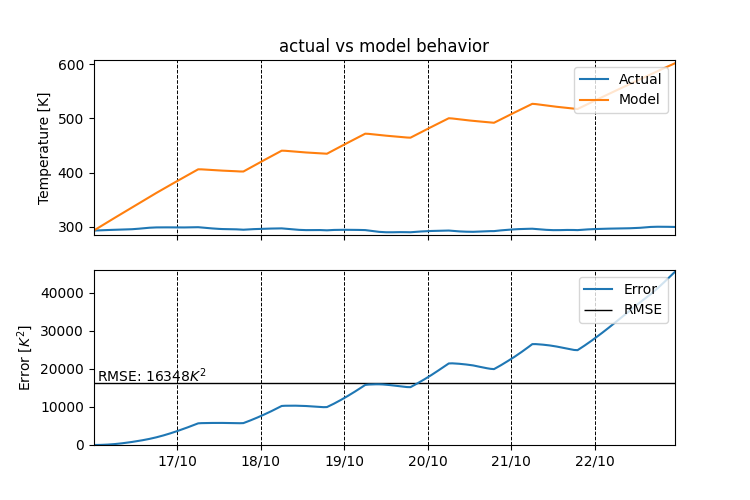
\includegraphics[scale=0.75]{images/error_actualvsmodel.png}
\caption{Predicted temperature model $\tilde{T}_{z}$ vs Actual temperature $T_z$ }
\label{fig:Model Error}
\end{figure}
The tool used to solve this optimization problem was CasADi, which is an open-source software available for Python that allows numerical optimization and optimal control \cite{Andersson2018}. In the next lines, a brief explanation of the code is given, thereafter an interpretation of the results is shown. To begin, the function $\mathsf{minimize\_function}$ is defined. The first lines are used to create different pythons lists, to save the ambient temperature $T_a$, heat from solar radiation $\dot{Q}_{sun}$ and time. All these were retrieved from historical data. Next, two new arrays were created for the heat input from occupancy $\dot{Q}_{g}$, and for the heat from radiator $\dot{Q}_{h}$. Their values were assigned based on the assumptions stated on section \ref{subsec:zone_model}.

Subsequently, the optimization problem is presented in the next code snippet, and a brief explanation is given as follows:
\begin{enumerate}
  \itemsep0em 
  \item The collection class $\mathsf{Opti()}$ is initialized.
  \item Three decision variables (all of them scalar) are declared and vertically concatenate into the vector $\mathbf{p}$.
  \item The objective function $f$, is defined as a summation of all the sample errors.
  \item The objective function to minimize, is declared into the $\mathsf{Opti()}$ class, which involves all variables previously defined.
  \item An Interior Point OPTimizer (IPOPT) is selected as a solver.
  \item An initial guess is provided with the values proposed in Table \ref{tab:initial_guess}. If this line is not declared, a numerical zero would be assumed.
  \item After setting up the problem, a solve method is called. 

\end{enumerate}

\begin{python}
def minimize_function(Tz_a):
   
    # Initiating Optimization variables
    opti = Opti()
    R = opti.variable()
    C = opti.variable()
    gA = opti.variable()
    p = vertcat(R, C, gA)  # parameter vector

	  # Definition of Objective function
    Tz = 293.15  # Initial temperature guess
    f = 0   # Objective function initial value

    for i in range(N):
        f = f + (Tz - Tz_a[i]) ** 2
        Tz_next = delta_t * ((Qsun[i] * gA + Qh[i] + Qg[i]) / C + (temp[i] - Tz) / (R * C)) + Tz
        Tz = Tz_next
        
    f = f + (Tz - Tz_a[N - 1]) ** 2

	  # Objective function to minimize and Solver definition
    opti.minimize(f)
    opti.solver('ipopt')

    # Initial guess parameter vector
    p_hat = vertcat(R_guess, C_guess, gA_guess)
    opti.set_initial(p, p_hat)

	  # Solve method
    sol = opti.solve()

    return sol.value(p)
\end{python}
\newpage
After executing the code, the solver 'ipopt' found the optimal values in 14 iterations, in which the decision variable $\mathbf{p}$ got the next values assigned: 
\begin{align}
    \mathbf{p} &= \begin{bmatrix}
           \tilde{C}_z\\
           \tilde{R}_w \\
           \tilde{gA} 
         \end{bmatrix} = \begin{bmatrix}
           4999397.46\\
           0.0100\\
           0.9445 
         \end{bmatrix} 
  \end{align}
This values are approximately the same as the values used to build the correct model stated in Table \ref{tab:constants}, so it can be concluded that the optimal values were found correctly. In addition, we inspect the evolution of the error in Figure \ref{fig:Error Evolution}. It can be observed that the error it is almost equal to 0, hence the minimization of the function was obtained. Due to the scaling factor of the graph, the reader can be confused believing that the $\mathsf{Error = 0}$ was obtained in iteration 7, but the actual value in that iteration is in the order of magnitude $10^3$, which is still far from zero. In contrast, the value in the last iteration is in the $10^{-3}$ order, therefore, it is considered as the minimum value of the optimization problem.
\begin{figure}[H]
\centering
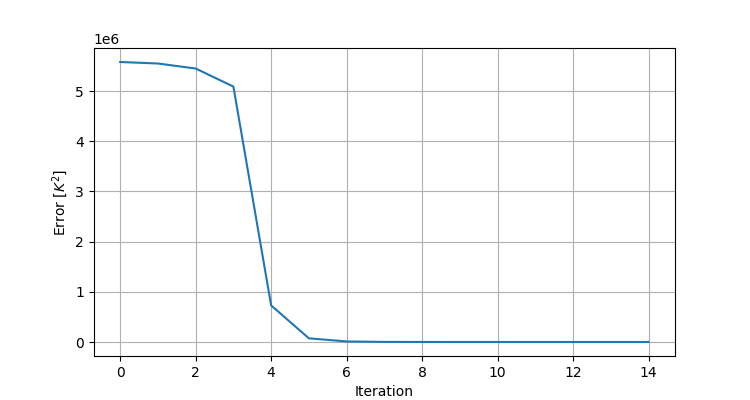
\includegraphics[scale=0.75]{images/Error_evolution.png}
\caption{Error evolution $[K^2]$ throughout each iteration}
\label{fig:Error Evolution}
\end{figure}